% Provenance (never printed): see sources/outline_sources.md (Year 3:
% ocean dynamics: the Ekman layer derived, the Sverdrup balance, western
% intensification, the abyssal circulation, ocean tides).
% Brief: sources/book5/BRIEFS.md, ch. 21. Curves from
% figdata/bachelor-3/wind_driven_gyre.py and tides.py. Exercise and problem
% values in the Book 5 scratch calculator calc/ch21.py. The basins, winds
% and stations of the exercises and the problem are invented.
\chapter{海洋动力学}\label{ch:b3:ocean-dynamics}

经佛罗里达海峡，墨西哥湾流向北输送的水量约
为 \qty{32}{\sverdrup}，并沿海岸北行时不断增大，
至北纬 \ang{40} 附近约达 \qty{150}{\sverdrup}。同一大洋的另一侧，葡萄牙和北非近海
没有与之相似的水流向南：墨西哥湾流北输的水，
向赤道回流，形成缓慢而宽广的漂流，横跨数千
千米的开阔海域。北半球每个大洋盆地都呈相同的不对称形态，
其快速洋流位于西侧。这一不对称
源于风、海水的摩擦，以及地球的一个事实：
科里奥利参数向极地方向增大。
% ledger: rapid:transports (31.7 Sv, rounded), stewart:north-atlantic

\begin{recall}
月球与太阳的引潮力、大潮与小潮，均见于物理学教材。风应力、埃克曼层、埃克曼输送与
埃克曼螺旋、上升流与下降流、
环流、西
边界流、斯韦德鲁普（$\qty{1}{\sverdrup} =
\qty{e6}{m^3/s}$），经向翻转环流与深层水的形成，
均见于本科一年级分册中的海洋环流一章；
那里风应力记作 $\vec T$，此处记作
$\vec\tau$。科里奥利参数、$\beta$ 平面、罗斯贝半径
和地转平衡见于第~\ref{ch:b3:gfd-foundations}~章；
涡度与\omterm{def:b3:atmospheric-dynamics:pv}{位涡}见于第~\ref{ch:b3:atmospheric-dynamics}~章。
\end{recall}

\section{埃克曼层的推导}\label{sec:b3:ocean-dynamics:ekman}

在本科一年级分册中，埃克曼输送由整层的受力平衡求得，
层内速度的螺旋则只作了陈述。
在涡黏性系数 $A_z$ 为常数的湍流摩擦下，螺旋可由
方程在几行内推出。把水平速度写成复数
$W = u + \mathrm iv$，风应力写成 $\tau =
\tau_x + \mathrm i\tau_y$；乘以 $-\mathrm i$ 相当于将矢量
顺时针旋转 \ang{90}，即从上方看时转到其右侧。

\begin{theorem}[稳定风驱动表层的速度剖面]\label{thm:b3:ocean-dynamics:ekman}
在定常、水平均匀、深度很大且密度为常数
$\rho$ 的海洋中，垂向涡黏性系数 $A_z$ 为常数，科里奥利参数
$f > 0$，风应力 $\tau$ 驱动的海流为
\[
W(z) = W_0\,\mathrm e^{(1+\mathrm i)z/\delta},\qquad
W_0 = \frac{\tau}{\rho\sqrt{fA_z}}\,\mathrm e^{-\mathrm i\pi/4},\qquad
\delta = \sqrt{\frac{2A_z}{f}} ,
\]
对 $z \le 0$，表层海流较风应力向右偏转 \ang{45}。
随深度增加，海流进一步向右偏转，并按 $\mathrm
e^{z/\delta}$ 衰减；总输送 $\int_{-\infty}^0 W\,\mathrm dz =
-\mathrm i\tau/(\rho f)$ 与风应力右侧方向成直角。
\end{theorem}

\begin{proof}
远离海岸时该层内无水平压强梯度，
科里奥利力与摩擦力平衡：$-fv = A_z u''$ 与 $fu =
A_z v''$，撇号表示对 $z$ 的导数。将第二式乘以
$\mathrm i$ 后相加，得 $A_zW'' = \mathrm ifW$。其解为
$\mathrm e^{\pm(1+\mathrm i)z/\delta}$，因为 $(1+\mathrm i)^2/\delta^2 =
2\mathrm i/\delta^2 = \mathrm if/A_z$；只有正号在
$z \to -\infty$ 时保持有界。表层应力由摩擦力承担，
$\rho A_zW'(0) = \tau$，故 $W_0 = \tau\delta/(\rho A_z(1+\mathrm i))$。
由 $\delta/(\sqrt2 A_z) = 1/\sqrt{fA_z}$ 及 $1/(1+\mathrm i) = \mathrm
e^{-\mathrm i\pi/4}/\sqrt2$，即得所述的 $W_0$。因子
$\mathrm e^{\mathrm iz/\delta}$ 随 $z$ 减小而顺时针转动。最后
$\int_{-\infty}^0 W\,\mathrm dz = W_0\delta/(1+\mathrm i) =
\tau\delta^2/(\rho A_z(1+\mathrm i)^2) = \tau\delta^2/(2\mathrm i\rho A_z)
= -\mathrm i\tau/(\rho f)$.
\end{proof}

该定理重现了本科一年级分册中的两个结果：埃克曼的表层海流
偏转 \ang{45}，以及输送 $\tau/(\rho f)$，其方向与风应力成直角，
且与 $A_z$ 无关，而这一量向来难以准确测定。在
深度 $\pi\delta$ 处，海流与表层海流方向相反，
大小减小为表层的 $\mathrm e^{-\pi}$ 倍，即 \qty{4}{\percent}。

\begin{definition}[埃克曼深度；埃克曼抽吸]\label{def:b3:ocean-dynamics:ekman-pumping}
称\emph{埃克曼深度}\index{埃克曼深度}为 $D_E = \pi\delta =
\pi\sqrt{2A_z/f}$，即埃克曼螺旋中海流与表层海流方向相反的
深度；它度量埃克曼层的
厚度。称\emph{埃克曼抽吸}\index{埃克曼抽吸}为
由埃克曼输送的辐合或辐散所强迫、位于埃克曼层底的垂向速度 $w_E$：
输送辐合处向下，
辐散处向上，有时称为埃克曼吸力。
\end{definition}

\begin{proposition}[埃克曼抽吸]\label{prop:b3:ocean-dynamics:pumping}
若海面处垂向速度为零，则\omterm{def:b3:ocean-dynamics:ekman-pumping}{埃克曼抽吸}为
\[
w_E = \operatorname{curl}_z\frac{\vec\tau}{\rho f}
= \frac{1}{\rho f}\Big(\frac{\partial\tau_y}{\partial x} -
\frac{\partial\tau_x}{\partial y}\Big) + \frac{\beta\tau_x}{\rho f^2} ,
\]
向上为正。
\end{proposition}

\begin{proof}
该层的体积输送为 $(U_E, V_E) = (\tau_y,
-\tau_x)/(\rho f)$，即定理的分量形式。对
连续性方程 $\partial w/\partial z = -(\partial u/\partial x +
\partial v/\partial y)$ 沿层积分，得 $w(0) - w_E = -(\partial
U_E/\partial x + \partial V_E/\partial y)$，故 $w_E = \partial_x(\tau_y/\rho
f) - \partial_y(\tau_x/\rho f)$。利用 $\mathrm df/\mathrm dy =
\beta$ 展开即得第二种形式。
\end{proof}

海面上气旋式旋转、旋度为正的风，会把
层下的水抽升上来，反气旋式的风则把水压下。在副热带
海洋上，信风从东方吹来，位于
赤道一侧，西风带则从西方吹来，位于极地一侧。二者的埃克曼
输送，信风下方指向北，西风下方指向南，
在两者之间汇聚：表层水堆积并被压入下方，如
下图所示。沿海岸，当
风以海岸位于其左侧的方向吹（北半球）时，输送
离开岸边，本科一年级分册所说的沿岸上升流
即集中于岸壁的\omterm{def:b3:ocean-dynamics:ekman-pumping}{埃克曼抽吸}。

\begin{omfigure}
\centering
\begin{tikzpicture}[>=stealth, font=\small, x=1.1cm, y=1cm]
\fill[omThm!7] (-5,0) rectangle (5,-3.6);
\draw[thick] (-5,0) -- (5,0);
\draw[black!45, densely dashed] (-5,-0.9) -- (5,-0.9);
\node[font=\scriptsize, black!60, anchor=north east, inner sep=1pt] at (4.95,-0.95) {埃克曼层};
% winds: west is out of the page, east into the page
\foreach \x in {-4.2,-3.4,-2.6} {\draw (\x,0.55) circle (0.13); \fill (\x,0.55) circle (0.04);}
\foreach \x in {2.6,3.4,4.2} {\draw (\x,0.55) circle (0.13);
  \draw (\x-0.09,0.46) -- (\x+0.09,0.64); \draw (\x-0.09,0.64) -- (\x+0.09,0.46);}
\node[above] at (-3.4,0.75) {信风，从东方吹来};
\node[above] at (3.4,0.75) {西风带，从西方吹来};
% Ekman transports converge
\draw[->, omDef, very thick] (-4.5,-0.45) -- (-1.2,-0.45);
\draw[->, omDef, very thick] (4.5,-0.45) -- (1.2,-0.45);
\node[omDef, font=\scriptsize, fill=omThm!7, inner sep=1pt] at (-2.85,-0.72) {埃克曼输送};
% pumping
\foreach \x in {-0.6,0,0.6} \draw[->, omThm, thick] (\x,-0.55) -- (\x,-1.55);
\node[omThm, font=\scriptsize, anchor=west] at (0.75,-1.25) {$w_E < 0$};
% squashed column and Sverdrup flow
\draw[thick, black!70] (-0.62,-1.75) rectangle (0.62,-3.1);
\node[font=\scriptsize, black!70, align=center] at (0,-2.42) {水柱 \\压扁};
\draw[->, omMeth, very thick] (-0.75,-2.42) -- (-3.2,-2.42);
\node[omMeth, font=\scriptsize, align=center, above] at (-2.6,-2.40) {斯韦德鲁普流，\\指向赤道};
\draw[black!45, densely dashed] (-5,-3.3) -- (5,-3.3);
\node[font=\scriptsize, black!60, anchor=south east, inner sep=1pt] at (4.95,-3.28) {风生流底部};
\node[below, font=\scriptsize] at (-5,-3.6) {南};
\node[below, font=\scriptsize] at (5,-3.6) {北};
\end{tikzpicture}

\par\smallskip{\small 北半球副热带环流的南北向剖面，
东向指入纸面。信风与西风带之下的埃克曼输送
汇聚，水被压向下方，而其下方的
水柱被压扁后向赤道移动，那里 $f$ 较小，
以保持其\omterm{def:b3:atmospheric-dynamics:pv}{位涡}。}\label{fig:b3:ocean-dynamics:pumping}
\end{omfigure}

\section{斯韦德鲁普平衡}\label{sec:b3:ocean-dynamics:sverdrup}

埃克曼层以下，海洋处于地转状态。一段水柱
受\omterm{def:b3:ocean-dynamics:ekman-pumping}{埃克曼抽吸}压扁后，为保持其\omterm{def:b3:atmospheric-dynamics:pv}{位涡} $f/h$，必须
向 $f$ 较小处移动，即向赤道。1947 年，H.~U.~斯韦德鲁普
使这一论证定量化，适用于风生流的全部深度。
% ledger: stewart:ekman-layer (Sverdrup 1947)

\begin{theorem}[斯韦德鲁普平衡]\label{thm:b3:ocean-dynamics:sverdrup}
在定常海洋中，非线性项与侧向摩擦
均可忽略，埃克曼层以下的内部为地转的，并且
在某深度 $-H$ 处竖直速度为零，则风生流单位宽度的
向北总体积输送满足\emph{斯韦德鲁普
平衡}\index{斯韦德鲁普平衡}
\[
\beta V = \frac{1}{\rho}\operatorname{curl}_z\vec\tau
= \frac{1}{\rho}\Big(\frac{\partial\tau_y}{\partial x} -
\frac{\partial\tau_x}{\partial y}\Big) .
\]
\end{theorem}

\begin{proof}
地转内部中 $fv_g = \rho^{-1}\partial p/\partial x$，且
$fu_g = -\rho^{-1}\partial p/\partial y$。由此 $\partial_x(fu_g) +
\partial_y(fv_g) = 0$，即 $f(\partial_xu_g + \partial_yv_g) + \beta
v_g = 0$，并由连续性，$\beta v_g = f\,\partial w/\partial z$。
自 $-H$（$w = 0$ 处）积分至埃克曼层底，
此处 $w = w_E$，得 $\beta V_g = fw_E$。由
\cref{prop:b3:ocean-dynamics:pumping}可知，$fw_E = \rho^{-1}\operatorname{curl}_z
\vec\tau + \beta\tau_x/(\rho f)$。加上埃克曼输送 $V_E =
-\tau_x/(\rho f)$，乘以 $\beta$，抵消最后一项：
$\beta(V_g + V_E) = \rho^{-1}\operatorname{curl}_z\vec\tau$。
\end{proof}

该平衡的特别之处在于它无需下列要素：既不需要流动的深度，
也不需要其竖直结构、涡动黏性，只需要
风的旋度与 $\beta$。斯韦德鲁普从运动方程
积分至无运动深度导出了它，并用
科考船\emph{Carnegie}与
\emph{Bushnell}的水文断面检验，位于东热带太平洋，介于北纬\ang{34}与
南纬\ang{10}，无运动深度取为\qty{1000}{m}：由风算出的输送
与由密度场算出的输送相符，即使
在洋流逆风的地方亦然。后来采用更好风场资料的研究
发现无运动深度接近\qty{500}{m}时吻合最佳，而且
1999 年对赤道太平洋平均应力的测量发现那里的
流动满足\omterm{thm:b3:ocean-dynamics:sverdrup}{斯韦德鲁普平衡}。该平衡能否处处成立，
比假定它成立更难证明：几乎所有海洋环流理论
都以它为出发点。
% ledger: stewart:sverdrup

取本章习题中的虚构盆地：介于北纬\ang{20}与
\ang{50}之间，宽\qty{6000}{km}，受纬向应力 $\tau_x =
-\tau_0\cos(\pi(\varphi - \ang{20})/\ang{30})$，其中 $\tau_0 =
\qty{0.1}{Pa}$，北纬\ang{20}处为东风，北纬\ang{50}处为西风，
北纬\ang{35}处为零。盆地几乎全部区域应力旋度为负：
海水被压下，北纬\ang{35}处每年下压约\qty{35}{m}，并
内部向南流动，北纬\ang{35}处每米宽的输送为\qty{4.9}{m^2/s}，
横跨整个盆地共\qty{29.4}{\sverdrup}。由观测风场算出，
北大西洋副热带环流的斯韦德鲁普输送约达
\qty{30}{\sverdrup}，位于北纬\ang{28}附近。
% ledger: stewart:north-atlantic (computed in figdata/bachelor-3/wind_driven_gyre.py)

\begin{omfigure}
\begin{tikzpicture}
\begin{groupplot}[group style={group size=3 by 1, horizontal sep=0.45cm, yticklabels at=edge left},
  width=0.37\linewidth, height=0.46\linewidth, ymin=20, ymax=50, ytick={20,25,30,35,40,45,50},
  tick label style={font=\scriptsize}, label style={font=\small}, title style={font=\small}]
\nextgroupplot[xlabel={$\tau_x$ (\unit{Pa})}, ylabel={北纬（\unit{\degree}）},
  xmin=-0.12, xmax=0.12, xtick={-0.1,0,0.1}, title={风应力},
  scaled x ticks=false, xticklabel style={/pgf/number format/fixed}]
% computed in figdata/bachelor-3/wind_driven_gyre.py
\addplot[black!50, thin] coordinates {(0,20) (0,50)};
\addplot[omThm, thick] table[x=tau, y=lat] {figdata/out/bachelor-3-wind_driven_gyre-merid.dat};
\nextgroupplot[xlabel={$w_E$ (\unit{m/\text{年}})}, xmin=-45, xmax=12, xtick={-40,-20,0},
  title={埃克曼抽吸}]
\addplot[black!50, thin] coordinates {(0,20) (0,50)};
\addplot[omDef, thick] table[x=wE, y=lat] {figdata/out/bachelor-3-wind_driven_gyre-merid.dat};
\nextgroupplot[xlabel={输送 (\unit{\sverdrup})}, xmin=-32, xmax=10, xtick={-30,-20,-10,0,10},
  title={斯韦德鲁普}]
\addplot[black!50, thin] coordinates {(0,20) (0,50)};
\addplot[omMeth, thick] table[x=Vtot, y=lat] {figdata/out/bachelor-3-wind_driven_gyre-merid.dat};
\end{groupplot}
\end{tikzpicture}

\par\smallskip{\small 题中虚构的盆地，自北纬\ang{20}至
\ang{50}，宽\qty{6000}{km}。左图为纬向风应力，向东为正；
中图为\omterm{def:b3:ocean-dynamics:ekman-pumping}{埃克曼抽吸}，向上为正：海水被压下，
在北纬\ang{47}以南，南部最强，此处 $f$ 较小，
其以北则被抽升。右图为横跨盆地的向北斯韦德鲁普输送总量：
内区向南流动，北纬\ang{35}处为\qty{29.4}{\sverdrup}，
但北缘一条狭窄的带除外，该处应力旋度变号。}\label{fig:b3:ocean-dynamics:sverdrup}
\end{omfigure}
% ledger: earth:Rmean, geod5:grs80-defining

斯韦德鲁普输送在每一点上确定了 $V$，但流函数
需要边界条件，而经向壁面只能施加一个。若
内区在东边界处满足无穿越流，则向南的流
在西边界处无处可去；质量须由一股洋流送回，
而这股洋流是无摩擦的斯韦德鲁普方程所无法描述的。

\section{西向强化}\label{sec:b3:ocean-dynamics:western}

1948 年，H.~斯托梅尔在最简单的海洋中加入了最简单的摩擦，并
发现回流挤向西边界，如
本科一年级分册中他的环流图所示。他只在科里奥利
参数随纬度向北增大时才得到此结果：无自转，或参数均匀时，
他的环流是对称的。
% ledger: stewart:stommel, stommel:1948

\begin{definition}[西向强化；斯托梅尔模型；芒克边界层]\label{def:b3:ocean-dynamics:western-intensification}
\emph{西向强化}\index{西向强化}指风生环流的回流
被挤入紧靠盆地西侧的狭窄快速洋流。
\emph{斯托梅尔
模型}\index{斯托梅尔模型}是矩形盆地中深度恒定的均匀海洋，
由纬向风应力驱动，并受底部摩擦减慢，其与深度积分速度成正比，
摩擦速率为 $r$；其输送流函数 $\psi$
（$U = -\partial\psi/\partial y$, $V =
\partial\psi/\partial x$）满足
\[
r\nabla^2\psi + \beta\frac{\partial\psi}{\partial x} =
\frac{1}{\rho}\operatorname{curl}_z\vec\tau ,\qquad \psi = 0 \text{ 在边界上.}
\]
\emph{芒克边界层}\index{芒克边界层}是同一环流的西边界层，
在侧向涡黏度 $A_H$ 代替底部摩擦时，
其宽度尺度为 $\delta_M =
(A_H/\beta)^{1/3}$。
\end{definition}

该方程即\omterm{thm:b3:ocean-dynamics:sverdrup}{斯韦德鲁普平衡}加上底部摩擦的旋度，
沿深度积分后为 $\beta V = \rho^{-1}\operatorname{curl}_z
\vec\tau - r\zeta_T$，其中 $\zeta_T = \nabla^2\psi$ 为
输送的涡度。

\begin{theorem}[斯托梅尔环流的西边界层]\label{thm:b3:ocean-dynamics:stommel}
在盆地 $0 \le x \le X$，$0 \le y \le L$ 中，设 $\tau_x = -\tau_0
\cos(\pi y/L)$ 且 $\delta_S = r/\beta \ll X$ 时，斯托梅尔流函数
在 $\delta_S/X$ 的首阶近似下为
\[
\psi = A\sin\frac{\pi y}{L}\Big[(X - x) - X\mathrm e^{-x/\delta_S}\Big],
\qquad A = \frac{\pi\tau_0}{\rho\beta L} .
\]
内区向南输送 $AX\sin(\pi y/L)$；紧靠西边界、宽为
$\delta_S$ 的边界层将其送回北方；东边界处不能
存在边界层。
\end{theorem}

\begin{proof}
应力旋度为 $-\partial\tau_x/\partial y = -(\pi\tau_0/L)\sin(\pi
y/L)$。在盆地宽度上，摩擦项比
$\beta$ 项小 $\delta_S/X$ 倍，略去后得\omterm{thm:b3:ocean-dynamics:sverdrup}{斯韦德鲁普平衡}，
$\beta\,\partial\psi/\partial x = -(\pi\tau_0/\rho L)\sin(\pi y/L)$，
其在 $x = X$ 处为零的解为 $\psi_I = A\sin(\pi y/L)(X - x)$。它在
$x = 0$ 处并不为零。近壁处 $\psi$ 随 $x$ 快速变化，
方程对修正量化为 $r\,\partial^2\psi/\partial x^2 + \beta\,\partial\psi/
\partial x = 0$，其解为常数与
$\mathrm e^{-x/\delta_S}$。该解向东衰减，远离西边界。
加上 $-AX\sin(\pi y/L)\,\mathrm e^{-x/\delta_S}$ 使 $\psi = 0$
于 $x = 0$ 处，且不改变内区。在东边界处，
修正项须向西衰减，远离 $x = X$，
而 $\mathrm e^{-x/\delta_S}$ 向西增长：不存在这样的层，因此
内区必须自行满足东边界条件，如 $\psi_I$ 所示。
向北的输送介于壁面与 $V$ 变号之处之间，
即该处的 $\psi$，接近 $AX\sin(\pi y/L)$。
\end{proof}

同一结论也可由涡度得出。在内区，风使每一列获得负涡度，
该列通过向南移动来偿付，
移向较小的 $f$。返回北方时它获得\omterm{def:b3:atmospheric-dynamics:vorticity-kinds}{行星涡度}，
而必须失去它，这只能靠摩擦完成。在一股向北的洋流中，
其流速自西边界附近向东递减，$\partial
v/\partial x < 0$，在其宽度的大部分上成立：洋流的涡度为负，而摩擦作用于它，
提供各列所需的正涡度。一股向北的
紧靠东边界的向北洋流涡度为正，
摩擦则会去掉错误的符号。

\begin{omfigure}
\begin{tikzpicture}
\begin{groupplot}[group style={group size=2 by 1, horizontal sep=1.7cm},
  width=0.48\linewidth, height=0.42\linewidth, xmin=0, xmax=400,
  xlabel={离西边界的距离 (\unit{km})},
  tick label style={font=\scriptsize}, label style={font=\small},
  legend style={font=\scriptsize, draw=none, fill=none}]
\nextgroupplot[ylabel={$V$ (\unit{m^2/s})}, ymin=-80, ymax=600, legend pos=north east,
  legend cell align=left]
% computed in figdata/bachelor-3/wind_driven_gyre.py
\addplot[omThm, thick] table[x=x, y=vS] {figdata/out/bachelor-3-wind_driven_gyre-bl.dat};
\addlegendentry{斯托梅尔，$\delta_S = \qty{53}{km}$}
\addplot[omDef, thick] table[x=x, y=vM] {figdata/out/bachelor-3-wind_driven_gyre-bl.dat};
\addlegendentry{芒克，$\delta_M = \qty{64}{km}$}
\addplot[black!50, thin, forget plot] coordinates {(0,0) (400,0)};
\nextgroupplot[ylabel={距边界的输运 (\unit{\sverdrup})}, ymin=0, ymax=36,
  legend pos=south east, legend cell align=left]
\addplot[omThm, thick] table[x=x, y=cS] {figdata/out/bachelor-3-wind_driven_gyre-bl.dat};
\addlegendentry{斯托梅尔}
\addplot[omDef, thick] table[x=x, y=cM] {figdata/out/bachelor-3-wind_driven_gyre-bl.dat};
\addlegendentry{芒克}
\addplot[black!60, densely dashed] coordinates {(0,29.4) (400,29.4)};
\addlegendentry{内区，\qty{29.4}{\sverdrup}}
\end{groupplot}
\end{tikzpicture}

\par\smallskip{\small 题中虚构海盆中部的西边界层，
即北纬 \ang{35}、宽 \qty{6000}{km} 的海盆。左图为单位宽度的向北输运：
斯托梅尔层在底摩擦
$r = \qty{e-6}{s^{-1}}$ 的作用下从边界处指数衰减；芒克层取
$A_H = \qty{5e3}{m^2/s}$，边界处无滑移，从零开始上升，
在约 \qty{80}{km} 处达到峰值，其后跟随一股弱的向南逆流。
右图为边界与各距离之间的输运，
与内区向南输送的 \qty{29.4}{\sverdrup} 相比较：斯托梅尔层
在其流动转向南方之前聚集 \qty{27.9}{\sverdrup}，芒克喷流
在其逆流出现之前聚集 \qty{33.0}{\sverdrup}。}\label{fig:b3:ocean-dynamics:boundary}
\end{omfigure}
% ledger: stewart:munk

取北纬 \ang{35}，$r = \qty{e-6}{s^{-1}}$，$\delta_S = \qty{53}{km}$，并且
向北流动占据离边界的前 \qty{250}{km}。1950 年，
W.~H.~芒克以侧向涡黏性 $A_H$ 取代底摩擦，
它作用于洋流内部的切变；方程增加一项
$A_H\nabla^4\psi$，在西边界附近，修正项
变为 $\mathrm e^{-x/2\delta_M}$ 乘以振荡项
$\cos(\sqrt3x/2\delta_M)$ 与 $\sin(\sqrt3x/2\delta_M)$。取 $A_H = \qty{5e3}{m^2/s}$，
向北喷流宽约 \qty{225}{km}（图中海盆内为 \qty{233}{km}），
其外侧伴有弱的逆流，
形状接近墨西哥湾流和黑潮。与斯托梅尔层相同，
喷流的输运不依赖摩擦，
只取决于风应力旋度、海盆宽度和 $\beta$。依据其时代的风场，芒克算得墨西哥湾流为 \qty{36}{\sverdrup}，
黑潮为 \qty{39}{\sverdrup}，约为当时实测输运的一半；
采用更好的拖曳系数和更精细的应力平均，
1978 年得到墨西哥湾流为 \qty{32}{\sverdrup}。
主要借助海底电缆测量，佛罗里达海峡中的墨西哥湾流
自 2004 年起平均输运 \qty{31.7}{\sverdrup}。在下游，
它在北纬 \ang{40} 附近增至约 \qty{150}{\sverdrup}；
在哈特拉斯角近海，一股强烈的再循环流
打破了二者的吻合，而线性理论并不包含这一流动。
% ledger: stewart:munk, rapid:transports, stewart:north-atlantic

\section{深层环流}\label{sec:b3:ocean-dynamics:abyssal}

深海由少数几处区域补充。在本科一年级分册中，深层水
形成于北大西洋远端及南极周围，那里的表层水被冷却并变得致密，
随后以北大西洋深层水和南极底层水的形式在各海盆中扩散。
1958 年至 1960 年间，
H.~斯托梅尔、A.~B.~阿朗斯和 A.~J.~法勒探讨了它的扩散方式，
运用与斯韦德鲁普相同的涡度论证。

\begin{definition}[斯托梅尔–阿朗斯模型]\label{def:b3:ocean-dynamics:abyssal}
深层环流的\emph{斯托梅尔–阿朗斯模型}\index{斯托梅尔–阿朗斯模型}假定：深层水由少数
高纬度源地的对流补给，
它以缓慢、均匀的上升流 $W_0$ 经温跃层底部
回到上层海洋，并由热量的向下混合所平衡；
内区的流动为地转流，且守恒\omterm{def:b3:atmospheric-dynamics:pv}{位涡}，
环流由深层西边界
流闭合。
\end{definition}

\begin{proposition}[深渊内区的极向流动]\label{prop:b3:ocean-dynamics:abyssal}
在\omterm{def:b3:ocean-dynamics:abyssal}{斯托梅尔–阿朗斯模型}中，于平坦海底之上，深渊内区经深度积分的
向北输运为
\[
V = \frac{f}{\beta}W_0 = a\tan\varphi\,W_0 ,
\]
当 $W_0 > 0$ 时，两个半球内的输运均指向极地。
\end{proposition}

\begin{proof}
在地转内区中，$\beta v = f\,\partial w/\partial z$，与
\omterm{thm:b3:ocean-dynamics:sverdrup}{斯韦德鲁普平衡}的证明相同。自平坦海底（$w = 0$）积分至
深渊层顶（$w = W_0$），得 $\beta V =
fW_0$，且 $f/\beta = 2\Omega\sin\varphi\,a/(2\Omega\cos\varphi) =
a\tan\varphi$。在南半球 $\tan\varphi < 0$：流动向南，
同样指向极地。
\end{proof}

这一结果有违直觉：深渊内区的流动指向
源地，而非背离源地。斯托梅尔与阿朗斯建造了旋转水槽实验
以说服自己。源地来的水沿西边界行进，
以深层西边界流的形式前进，并在途中补给
内区。在赤道与极地之间的一段洋区中，
若全部源地水量 $S_0$ 位于极地附近，西边界流
向赤道输送 $2S_0\sin\varphi$，即极地源量的两倍，
而在赤道处为零：超出 $S_0$ 的部分是来自内区的再循环水。
该模型表明，深层环流由混合驱动，
而非由下沉驱动：若无上升流，对流只会以
停滞的冷水池充满深渊。其转移时间从
源地附近的数百年，到北太平洋的近千年不等。
在真实的海底上，海岭分隔各海盆，混合
在粗糙地形之上十分强烈，深层流动也远比
模型中的更趋纬向。其持久的预言是深层西边界流：在
北大西洋，约 \qty{14}{\sverdrup} 的水体以
\qty{2}{\celsius} 南返，而墨西哥湾流则将暖水
北输。
% ledger: stewart:stommel-arons, stewart:deep-circulation, stewart:heat-conveyor

\begin{omfigure}
\centering
\begin{tikzpicture}[>=stealth, font=\small, scale=0.95]
\fill[omThm!7] (0,0) -- (7,0) -- (4.2,5) -- (2.8,5) -- cycle;
\draw[thick] (0,0) -- (2.8,5) -- (4.2,5) -- (7,0);
\draw[black!45, densely dashed] (0,0) -- (7,0);
\node[below, font=\scriptsize] at (3.5,0) {赤道};
\node[above, font=\scriptsize] at (3.5,5) {指向极地};
\fill[omThm] (3.05,4.6) circle (0.17);
\node[font=\scriptsize, anchor=west, inner sep=1pt] at (3.22,4.6) {$S_0$};
% western boundary current
\draw[->, omThm, very thick] (2.75,4.35) -- (0.35,0.25);
\node[omThm, font=\scriptsize, rotate=60.8, inner sep=1pt] at (0.85,2.45) {深层西边界流};
% interior poleward flow
\foreach \x/\y in {2.6/0.7, 3.8/0.7, 5.0/0.7, 3.1/1.7, 4.3/1.7, 3.6/2.7, 4.6/2.7} {
  \draw[->, omMeth, thick] (\x,\y) -- ++(0.15,0.65);}
% upwelling dots
\foreach \x/\y in {2.2/1.25, 3.4/1.25, 4.6/1.25, 5.6/1.25, 2.7/2.2, 3.9/2.2, 5.0/2.2, 3.3/3.2, 4.3/3.2, 3.8/3.9} {
  \draw[omDef] (\x,\y) circle (0.09); \fill[omDef] (\x,\y) circle (0.03);}
\node[omMeth, font=\scriptsize, align=left, anchor=west] at (6.45,2.6) {极向 \\内部流};
\node[omDef, font=\scriptsize, align=left, anchor=west] at (6.6,1.5) {上升流 $W_0$};
\end{tikzpicture}

\par\smallskip{\small 北半球海洋中一个扇区的斯托梅尔–阿朗斯深层环流，俯视图。
深水在近极地的源地 $S_0$ 处下沉，
经深层西边界流流向赤道，
并渗入向极方向流动的内部区域，
在整个区域内缓慢穿过温跃层上升
（图中圆点表示朝向读者的上升流）。}\label{fig:b3:ocean-dynamics:stommel-arons}
\end{omfigure}

模型的内部与 Sverdrup 的一样，是地转的，
深海的地转流所用的测量方法，与
Sverdrup 当年所用的相同：由密度求得。

\begin{definition}[动力计算法]\label{def:b3:ocean-dynamics:dynamic-height}
\emph{动力计算法}\index{动力计算法}利用两个水文站测得的密度，
计算两站之间的地转流。参考压强面上的流速取为零或已知，
两个等压面之间的\omterm{def:b3:gravity-geodesy:geopotential}{位势}距离 $\int\alpha\,\mathrm dp$（其中 $\alpha = 1/\rho$ 为比容），
分为两部分：两站相同的标准部分，
以及\emph{\omterm{def:b3:gravity-geodesy:geopotential}{位势}异常} $\Delta\Phi$；
上界面处的流速垂直于两站 $A$、$B$ 的连线，
两站相距 $L$，
流速
为：
\[
v = \frac{\Delta\Phi_B - \Delta\Phi_A}{fL} .
\]
\end{definition}

为什么不像气象学家那样直接测量压强？地转流的流速为
\qty{10}{cm/s}、位于 \ang{30} 纬度处时，所需压强梯度为
\qty{7.5e-3}{Pa/m}，即在 \qty{100}{km} 上相差 \qty{750}{Pa}，
相当于 \qty{7.4}{cm} 海水的重量。海底上没有任何压力计能够调平到这样的精度。
密度可精确到百万分之几，因而能够给出一个等压面
相对另一个等压面的倾斜。在北半球，较轻、较暖的水
位于顺流而下时的右侧。跨越墨西哥湾流，等密度面
的深度在 \qty{100}{km} 内变化
超过一千米。
% ledger: stewart:dynamic-method

\begin{method}[由两个站位计算地转流]\label{met:b3:ocean-dynamics:dynamic}
\begin{enumerate}
\item 在每个站位，计算比容异常 $\delta =
  \alpha(S, T, p) - \alpha(35, 0, p)$（由测得的盐度、
  温度和压强计算）。
\item 将其从参考压强积分到每个压强 $p$：
  $\Delta\Phi(p) = \int_p^{p_{\text{参考}}}\delta\,\mathrm dp$。
\item 在每个压强处，$v(p) = (\Delta\Phi_B - \Delta\Phi_A)/(fL)$ 即为
  相对参考面的流速，站位 $B$
  位于右侧时取正值。
\item 若参考面处的流速已知，则将其加上，数据可取自
  在该处漂移的浮标，或由卫星测得的海面坡度。
\end{enumerate}
\end{method}

\begin{inthefield}[一个浮标阵列]
\begin{minipage}[t]{0.52\linewidth}\vspace{0pt}
\begin{dated}{2024}
世界大洋中约有四千个 Argo 浮标在漂移。浮标由科考船舷侧放入，
下沉至约 \qty{1000}{m} 处漂移约九天；随后下沉至 \qty{2000}{m}，
再上浮至海面，上浮途中测量电导率、温度和压强，
循环约每十天一次。深层 Argo 浮标可剖面至 \qty{6000}{m}。
2024 年 7 月，该阵列收集了第三百万条剖面。
海洋学家由这些剖面，在每个浮标处计算\omterm{def:b3:ocean-dynamics:dynamic-height}{动力计算法}所需的
\omterm{def:b3:gravity-geodesy:geopotential}{位势}异常；浮标在两次浮出水面之间的位移，
给出其驻留深度处的平均流速，
Sverdrup 不得不假定的参考流速，
如今已能测得。
\end{dated}
\end{minipage}\hfill
\begin{minipage}[t]{0.44\linewidth}\vspace{0pt}
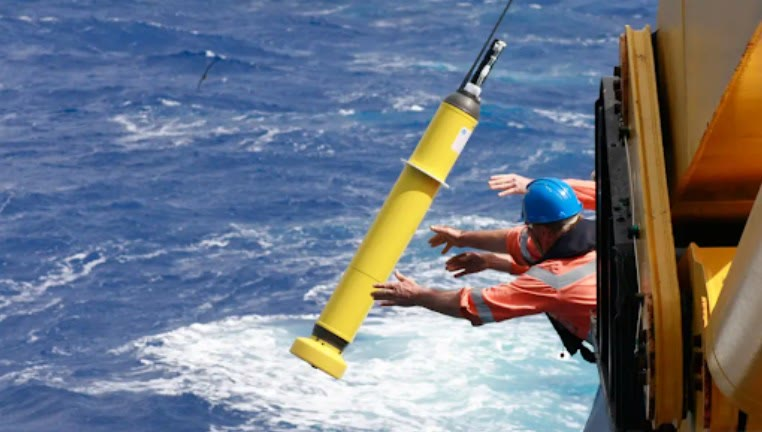
\includegraphics[width=\linewidth]{images/book5/b3-argo-deploy.jpg}

{\scriptsize 从科考船舷侧放入的一个 Argo 浮标（NOAA
Global Ocean Monitoring and Observing Program，公有领域）。}
\end{minipage}
\end{inthefield}
% ledger: argo:fleet, noaa:argo-25, photo:b3-argo-deploy

\section{海洋潮汐}\label{sec:b3:ocean-dynamics:tides}

海面每天涨落两次，每天的涨落时刻比前一天约晚不到一小时。
物理学教材解释了潮汐力：月球的引力
在地球近月一侧比地心处强，在远月一侧较弱，
因此相对于地心，水体在两侧都沿着
通向月球的连线被拉出。

\begin{definition}[平衡潮；分潮]\label{def:b3:ocean-dynamics:tides}
\emph{平衡潮}\index{平衡潮}是指覆盖整个地球的海洋表面，
若其瞬时跟随引潮势、不计惯性时所取的形状。一个\emph{分
潮}\index{分潮}是调和项之一，每一项的频率固定，由月球和太阳的运动决定，
其振幅和位相随地点而定，所有项之和即为潮汐；
各分潮以一个字母和每日循环次数命名，
例如 M$_2$，
即主要太阴半日
分潮。
\end{definition}

\begin{theorem}[月球的平衡潮]\label{thm:b3:ocean-dynamics:equilibrium-tide}
设月球质量为 $M$，距地心距离为 $d$，
地球质量为 $M_E$，半径为 $a$，
则距月下点夹角为 $\theta$ 处的\omterm{def:b3:ocean-dynamics:tides}{平衡潮}为
\[
\eta = K\,\frac{3\cos^2\theta - 1}{2},\qquad
K = \frac{M}{M_E}\Big(\frac{a}{d}\Big)^3 a .
\]
\end{theorem}

\begin{proof}
月球在距地心为 $a$、与地心连线夹角为 $\theta$ 的点处的势
为 $-GM/s$，其中 $s^2 = d^2 - 2ad\cos\theta +
a^2$。按 $a/d$ 展开，$1/s = (1/d)[1 + (a/d)\cos\theta + (a/d)^2
(3\cos^2\theta - 1)/2 + \cdots]$。第一项为常数；第二项为均匀场，
即使整个地球绕二者公共质心沿轨道加速运动的那一项，
对地球相对运动没有影响。
剩下的即为引潮势 $\Phi_T = -(GMa^2/d^3)(3
\cos^2\theta - 1)/2$。平衡时海面为总势的等势面，
$g\eta + \Phi_T = C$，其中 $g = GM_E/a^2$，于是
$\eta = (M/M_E)(a^4/d^3)(3\cos^2\theta - 1)/2 + C/g$。
$3\cos^2\theta - 1$ 在球面上的平均值为零；
水的体积固定，故 $C = 0$。
\end{proof}

取质量比 $0.0123$，$d = \qty{384400}{km}$，$a =
\qty{6371}{km}$，$K = \qty{0.357}{m}$：海面在月下点及其对跖点处高出 \qty{0.36}{m}，
在两者之间的大圆上则低 \qty{0.18}{m}，
总振幅为 \qty{0.54}{m}。在纬度 $\varphi$ 处，月球赤纬为 $\delta$、时角为 $H$，
则 $\cos\theta =
\sin\varphi\sin\delta + \cos\varphi\cos\delta\cos H$。地球在两个隆起之下自转，
某地每个太阴日（\qty{24}{h} \qty{50}{min}）经历两次高潮，
这就是半日潮。当月球
位于赤道以北或以南时，两个隆起发生倾斜，一天中的两次
高潮高度不等，如下图所示。太阳也引起一种
形式相同的潮汐，幅度为其 \num{0.46} 倍；朔望时两者叠加，
形成大潮，在上、下弦时则部分抵消。
% ledger: moon5:orbit, earth:Rmean, stewart:tide-equilibrium (computed in figdata/bachelor-3/tides.py)

\begin{omfigure}
\begin{tikzpicture}
\begin{groupplot}[group style={group size=2 by 1, horizontal sep=1.9cm},
  tick label style={font=\scriptsize}, label style={font=\small},
  legend style={font=\scriptsize, draw=none, fill=none}]
\nextgroupplot[width=0.40\linewidth, height=0.40\linewidth, axis equal image, hide axis,
  clip=false, xmin=-1.3, xmax=2.0, ymin=-1.25, ymax=1.25]
% computed in figdata/bachelor-3/tides.py
\addplot[fill=omThm!12, draw=omThm, thick] table[x=x, y=y] {figdata/out/bachelor-3-tides-bulge.dat};
\addplot[black, fill=black!10, domain=0:360, samples=91] ({cos(x)}, {sin(x)});
\draw[->, >=stealth, thick] (axis cs:1.25,0) -- (axis cs:1.95,0);
\node[above, font=\scriptsize, align=center] at (axis cs:1.6,0.08) {指向 \\月球};
\node[font=\scriptsize] at (axis cs:0,0) {地球};
\nextgroupplot[width=0.54\linewidth, height=0.40\linewidth, xlabel={时间 (\unit{h})},
  ylabel={$\eta$ (\unit{m})}, xmin=0, xmax=49.6, xtick={0,12,24,36,48}, ymin=-0.2, ymax=0.4,
  legend style={at={(axis cs:12.4,0.39)}, anchor=north}, legend cell align=left, legend columns=2]
\addplot[omDef, thick] table[x=t, y=eta0] {figdata/out/bachelor-3-tides-series.dat};
\addlegendentry{$\delta = 0$}
\addplot[omThm, thick] table[x=t, y=eta20] {figdata/out/bachelor-3-tides-series.dat};
\addlegendentry{$\delta = \ang{20}$}
\addplot[black!50, thin, forget plot] coordinates {(0,0) (49.6,0)};
\end{groupplot}
\end{tikzpicture}

\par\smallskip{\small 左图：月球的\omterm{def:b3:ocean-dynamics:tides}{平衡潮}，取包含月球的平面，
隆起放大约两百万倍。
右图：北纬 \ang{45} 处两个太阴日内的\omterm{def:b3:ocean-dynamics:tides}{平衡潮}，
月球位于赤道上（蓝色）及赤纬 \ang{20} 北（红色）时，
后一种情形下一次高潮明显高于另一次，
即日不等。}\label{fig:b3:ocean-dynamics:equilibrium-tide}
\end{omfigure}
% ledger: moon5:orbit, stewart:tide-constituents

对\omterm{def:b3:ocean-dynamics:tides}{平衡潮}作调和分析，即可得到其\omterm{def:b3:ocean-dynamics:tides}{分潮}。
其中最大的五个及其平衡振幅列于下表。
要预报某港口的潮汐，使误差小于其最大项的千分之一，至少需要 39 个\omterm{def:b3:ocean-dynamics:tides}{分潮}；
验潮站须连续记录超过 18.6 年，
即月潮调制的周期，方能将它们全部分离。

\begin{center}
\small
\begin{tabular}{llrr}
\hline
\omterm{def:b3:ocean-dynamics:tides}{分潮} & 成因 & 周期 (\unit{h}) & 平衡振幅 (\unit{m}) \\
\hline
M$_2$ & 主要太阴，半日 & \num{12.4206} & \num{0.2423} \\
S$_2$ & 主要太阳，半日 & \num{12.0000} & \num{0.1128} \\
N$_2$ & 月球椭率，半日 & \num{12.6584} & \num{0.0464} \\
K$_1$ & 日月合成，全日 & \num{23.9344} & \num{0.1416} \\
O$_1$ & 主要太阴，全日 & \num{25.8194} & \num{0.1005} \\
\hline
\end{tabular}
\end{center}
% ledger: stewart:tide-constituents, stewart:tide-prediction

实际潮汐并非\omterm{def:b3:ocean-dynamics:tides}{平衡潮}。若要使赤道上月下的隆起保持不动，
潮汐须在一个太阴日内绕地球一周，速度约为 \qty{460}{m/s}，
而只有深 \qty{22}{km} 的海洋中长重力波才能达到这一速度；
况且大陆会阻挡它。实际潮汐是一种受迫长波，
在各个海盆中近共振地摆动，
地球自转则使其绕盆地旋转。
% ledger: stewart:tide-prediction

\begin{definition}[开尔文波]\label{def:b3:ocean-dynamics:kelvin-wave}
海洋中的\emph{开尔文波}\index{开尔文波}是一种长重力波，
沿海岸或沿赤道传播，垂直于传播方向没有速度分量，
其波高随离岸距离按指数规律衰减，
特征尺度为罗斯贝半径。沿海岸传播时，北半球海岸位于其右侧，
南半球则位于其左侧。
\end{definition}

\begin{theorem}[沿岸开尔文波]\label{thm:b3:ocean-dynamics:kelvin}
设海洋水深 $H$ 均匀，位于 $f$ 平面上，$f > 0$，且以
沿 $y = 0$ 的直线海岸为界，海洋位于 $y > 0$ 一侧，线性浅水方程
在 $v = 0$ 时有如下解
\[
\eta = \mathrm e^{-y/L_R}F(x - ct),\qquad u = \frac{g}{c}\,\eta,\qquad
c = \sqrt{gH},\quad L_R = \frac{c}{f},
\]
对任意廓线 $F$ 成立，且在 $v = 0$ 时不存在沿
$-x$ 方向传播的解。
\end{theorem}

\begin{proof}
当 $v = 0$ 时，方程为 $\partial u/\partial t = -g\,\partial\eta/
\partial x$，$fu = -g\,\partial\eta/\partial y$，以及 $\partial\eta/\partial t
+ H\,\partial u/\partial x = 0$。由第一式与第三式可得 $\partial^2
\eta/\partial t^2 = gH\,\partial^2\eta/\partial x^2$：对 $x$ 而言，每条
$y = $ 常数的直线上都有波 $F(x \mp ct)$，其中 $c = \sqrt{gH}$，再由
第一式得 $u = \pm(g/c)\eta$。第二式变为 $\partial\eta/
\partial y = \mp(f/c)\eta$，故 $\eta \propto \mathrm e^{\mp y/L_R}$。取
上符号时波随离岸距离衰减；取下符号时波会
无界地伸入海洋，这是不允许的。波沿
$+x$ 方向传播，海洋位于其左侧，海岸位于其右侧。
\end{proof}

在深海中，水深 \qty{4000}{m}，$c = \qty{198}{m/s}$，
中纬度处的罗斯贝半径约为 \qty{2000}{km}：潮汐
绕整个海盆传播。在水深 \qty{50}{m} 的陆架海中，$c =
\qty{22}{m/s}$，罗斯贝半径小于 \qty{200}{km}，M$_2$
波长约为 \qty{1000}{km}。在海湾中，潮汐沿一侧海岸
以\omterm{def:b3:ocean-dynamics:kelvin-wave}{开尔文波}形式进入，并沿对岸返回，仍以海岸位于其右侧；
两列波在中间某些点相互抵消。

\begin{definition}[无潮点；同潮时线；等潮差线]\label{def:b3:ocean-dynamics:amphidrome}
\emph{无潮点}\index{无潮点}是某一\omterm{def:b3:ocean-dynamics:tides}{分潮}振幅为零的点，
其高潮绕该点旋转。\emph{同潮时线}\index{同潮时线}连接
某一\omterm{def:b3:ocean-dynamics:tides}{分潮}高潮同时到达的地点，
\emph{等潮差线}\index{等潮差线}连接潮差相等的地点。
同潮时线从无潮点向外辐射，
等潮差线则环绕无潮点。
\end{definition}

\begin{omfigure}
\centering
\begin{tikzpicture}
\begin{axis}[width=0.96\linewidth, height=0.35\linewidth, axis equal image,
  xmin=0, xmax=1600, ymin=0, ymax=400, xtick={0,400,800,1200,1600}, ytick={0,200,400},
  xlabel={沿河道距离（\unit{km}）}, ylabel={横向距离（\unit{km}）},
  tick label style={font=\scriptsize}, label style={font=\small}]
% computed in figdata/bachelor-3/tides.py
\addplot[omDef!70, densely dashed, unbounded coords=jump] table[x=x, y=y] {figdata/out/bachelor-3-tides-cor.dat};
\pgfplotsinvokeforeach{30,60,90,120,150,180,210,240,270,300,330}{
  \addplot[omThm, thin, unbounded coords=jump] table[x=x, y=y] {figdata/out/bachelor-3-tides-cot-#1.dat};
}
\addplot[omThm, very thick, unbounded coords=jump] table[x=x, y=y] {figdata/out/bachelor-3-tides-cot-0.dat};
\addplot[only marks, mark=*, mark size=2pt] table[x=x, y=y] {figdata/out/bachelor-3-tides-amph.dat};
\addplot[->, >=stealth, very thick, domain=20:310, samples=60] ({742.7+70*cos(x)}, {200+70*sin(x)});
\end{axis}
\end{tikzpicture}

\par\smallskip{\small 虚构河道中的两列 M$_2$ \omterm{def:b3:ocean-dynamics:tides}{分潮}\omterm{def:b3:ocean-dynamics:kelvin-wave}{开尔文波}，
河道宽 \qty{400}{km}，水深 \qty{50}{m}，位于北纬 \ang{55}，一列
沿南岸向东传播，另一列沿北岸向西传播。
红色为\omterm{def:b3:ocean-dynamics:amphidrome}{同潮时线}，每隔 \ang{30} 相位（约一小时）画一条，
粗线为时间零点时的高潮；蓝色虚线为\omterm{def:b3:ocean-dynamics:amphidrome}{等潮差线}，
每隔一列波在其海岸处振幅的五分之一画一条。
\omterm{def:b3:ocean-dynamics:amphidrome}{无潮点}（圆点）位于中心线上，彼此相隔半个波长，
即 \qty{495}{km}，高潮绕这些点按逆时针方向旋转
（箭头）。}\label{fig:b3:ocean-dynamics:amphidromes}
\end{omfigure}

由卫星测高得到的海洋潮汐图，在深海中精度约为
\qty{2}{cm}，处处显示出这一结构：M$_2$
潮峰绕北半球海盆的\omterm{def:b3:ocean-dynamics:amphidrome}{无潮点}逆时针旋转，
南半球则顺时针旋转，最大潮差出现在
海岸。潮汐耗散功率为 \qty{3.75}{TW}，其中 \qty{3.5}{TW}
发生在海洋中，约三分之二的 M$_2$ 能量耗散于陆架和浅海，
其余三分之一通过深海内波耗散。这部分能量
使日长每世纪增加约 \qty{2.07}{ms}，并使月球每年远离
地球约 \qty{3.86}{cm}；在深海中损失的那部分能量使海水混合，
为斯托梅尔–阿朗斯图景中驱动深层环流的那部分
混合提供能量。
% ledger: stewart:tide-prediction


\section{练习}

\begin{exercise}[$\star$]\label{exo:b3:ocean-dynamics:1}
在北纬 \ang{40} 处，一股风应力为 \qty{0.12}{Pa} 的西风吹过海面
($\rho = \qty{1025}{kg/m^3}$, $\Omega = \qty{7.292115e-5}{rad/s}$).
求每米宽度的埃克曼体积输送量及其方向，
以及长 \qty{1000}{km} 的断面上以斯韦德鲁普为单位的输送量。
\end{exercise}

\begin{exercise}[$\star$]\label{exo:b3:ocean-dynamics:2}
取 $A_z = \qty{0.05}{m^2/s}$，求北纬 \ang{45} 处的\omterm{def:b3:ocean-dynamics:ekman-pumping}{埃克曼深度}。
该深度处仍保留的表层流速比例是多少？
\end{exercise}

\begin{exercise}[$\star$]\label{exo:b3:ocean-dynamics:3}
在北纬 \ang{30} 处，风应力的旋度在一个
宽 \qty{5000}{km} 的海盆上为 \qty{-1e-7}{Pa/m}（$a = \qty{6371}{km}$）。求 $\beta$、
单位宽度的斯韦德鲁普输送量及总输送量，
并说明其方向。
\end{exercise}

\begin{exercise}[$\star$]\label{exo:b3:ocean-dynamics:4}
由 M$_2$ 与 S$_2$ 的周期，求大潮与小潮循环的
周期，即两种\omterm{def:b3:ocean-dynamics:tides}{分潮}两次对齐之间的
时间。
\end{exercise}

\begin{exercise}[$\star\star$]\label{exo:b3:ocean-dynamics:5}
西风应力从北纬 \ang{35} 处的 0 开始线性增大，至
北纬 \ang{45} 处的 \qty{0.1}{Pa}，该处位于其以北 \qty{1110}{km} 处。求
北纬 \ang{40} 处的\omterm{def:b3:ocean-dynamics:ekman-pumping}{埃克曼抽吸}，保留\cref{prop:b3:ocean-dynamics:pumping}中的两项，
以米每年计。水体是被向上还是向下推动？
\end{exercise}

\begin{exercise}[$\star\star$]\label{exo:b3:ocean-dynamics:6}
在斯托梅尔环流中，取 $r = \qty{2e-6}{s^{-1}}$ 且 $\beta =
\qty{2e-11}{m^{-1}.s^{-1}}$，求宽度 $\delta_S$。若边界
流在上层 \qty{800}{m} 中输送 \qty{30}{\sverdrup}，
位于宽度 $\delta_S$ 之内，其平均速度是多少？
\end{exercise}

\begin{exercise}[$\star\star$]\label{exo:b3:ocean-dynamics:7}
求芒克宽度 $\delta_M$ 及北向急流的宽度
$(2\pi/\sqrt3)\,\delta_M$，取北纬 \ang{30} 处、$A_H = \qty{e4}{m^2/s}$。若
$A_H$ 缩小为原来的八分之一，宽度如何变化？
\end{exercise}

\begin{exercise}[$\star\star$]\label{exo:b3:ocean-dynamics:8}
两个测站相距 \qty{80}{km}，沿由西（$A$）至东
（$B$）的方向位于北纬 \ang{36} 处。相对于 \qty{1000}{dbar} 面，
海面的\omterm{def:b3:gravity-geodesy:geopotential}{位势}异常在 $A$ 处为 \qty{14.5}{J/kg}，在
$B$ 处为 \qty{21.3}{J/kg}。求表层流相对于
\qty{1000}{dbar} 的流速及其方向。哪一个测站的水柱
更暖？
\end{exercise}

\begin{exercise}[$\star\star$]\label{exo:b3:ocean-dynamics:9}
考虑月球的\omterm{def:b3:ocean-dynamics:tides}{平衡潮}，$K = \qty{0.357}{m}$，并令
太阳潮与月球潮之比为 \num{0.46}，求\omterm{def:b3:ocean-dynamics:tides}{平衡潮}差
（天体下方的高潮减去距天体 \ang{90} 处的低潮），分别求大潮与
小潮时的值及其比值。
\end{exercise}

\begin{exercise}[$\star\star\star$]\label{exo:b3:ocean-dynamics:10}
在赤道的 $\beta$ 平面上，$f = \beta_0y$，其中 $\beta_0 =
2\Omega/a$。证明\omterm{def:b3:ocean-dynamics:kelvin-wave}{开尔文波} $\eta = G(y)F(x - ct)$、$v = 0$ 中的函数可化为
$G = \exp(-\beta_0y^2/2c)$，波被束缚在赤道两侧，
并向东传播。求其束缚尺度 $\sqrt{c/\beta_0}$，取
波速为 \qty{2.5}{m/s} 的波。
\end{exercise}

\begin{exercise}[$\star\star\star$]\label{exo:b3:ocean-dynamics:11}
(a)~推导深海内部的 $V = a\tan\varphi\,W_0$，依据 $\beta v =
f\,\partial w/\partial z$。(b)~取 $W_0 = \qty{e-7}{m/s}$，求 $V$ 在
北纬 \ang{30} 处的值，以及穿过海盆的总极向输送量，
海盆宽 \qty{5000}{km}。(c)~水体从何处补充？
\end{exercise}

\begin{exercise}[$\star\star\star$]\label{exo:b3:ocean-dynamics:12}
地转流 $W_g = u_g + \mathrm iv_g$ 流过平坦的海
床（位于 $z = 0$），涡动黏度为 $A_z$，海床处为无滑移。
(a)~证明 $W = W_g(1 - \mathrm e^{-(1+\mathrm i)z/\delta})$，$\delta =
\sqrt{2A_z/f}$。(b)~证明该底部埃克曼层的
输送亏损将竖直速度 $w = \tfrac12\delta\zeta_g$ 抽送至
内部，$\zeta_g$ 为地转流的涡度。(c)~对于
$A_z = \qty{0.01}{m^2/s}$，$f = \qty{e-4}{s^{-1}}$，且海洋
深 \qty{4000}{m}，求 $\delta$、旋转衰减率 $r =
f\delta/2H$，并以天为单位求其倒数。
\end{exercise}
% ledger: earth:Rmean, geod5:grs80-defining, stewart:tide-constituents, stewart:tide-equilibrium

\section{问题：阿马尔海中的一个环流}

\begin{problem}[{周末问题——埃克曼抽吸、斯韦德鲁普输送、
西边界流与一个虚构海洋的潮汐}]
\label{pb:b3:ocean-dynamics:1}
阿马尔海是一个虚构的海盆，为一矩形，北纬 \ang{20} 至
\ang{50}，宽 \qty{6000}{km}，深 \qty{4000}{m}。风应力为
纬向的，$\tau_x = -\tau_0\cos(\pi(\varphi - \ang{20})/\ang{30})$，其中 $\tau_0
= \qty{0.1}{Pa}$。取 $\rho = \qty{1025}{kg/m^3}$，$\Omega =
\qty{7.292115e-5}{rad/s}$，$a = \qty{6371}{km}$，$g = \qty{9.81}{m/s^2}$，
以及在需要 $\beta$ 平面时取北纬 \ang{35} 处的值。

\medskip\noindent\textbf{第一部分——埃克曼层。}
\begin{enumerate}
\item 求北纬 \ang{20}、\ang{35} 与 \ang{50} 处的风应力。
\item 求同纬度处的 $f$。
\item 求北纬 \ang{20} 及
  北纬 \ang{50} 处单位宽度的埃克曼体积输送，并给出其方向。海盆中的输送是
  汇聚还是发散？
\item 取 $A_z = \qty{0.05}{m^2/s}$，求北纬 \ang{35} 处的\omterm{def:b3:ocean-dynamics:ekman-pumping}{埃克曼深度}。
\item 求北纬 \ang{35} 处的\omterm{def:b3:ocean-dynamics:ekman-pumping}{埃克曼抽吸}，以米每秒及
  每年为单位。
\item 这一抽吸需多少年才能将表层水
  下压 \qty{500}{m}？
\end{enumerate}

\medskip\noindent\textbf{第二部分——斯韦德鲁普内部区。}
\begin{enumerate}[resume]
\item 求海盆由南至北的长度 $L$，以及
  北纬 \ang{35} 处的 $\beta$ 值。
\item 求北纬 \ang{35} 处风应力的旋度。
\item 求北纬 \ang{35} 处单位宽度的斯韦德鲁普输送，并给出其
  方向。
\item 求北纬 \ang{35} 处穿过海盆的内部总输送量，
  以斯韦德鲁普计。
\item 若该流分布于上层 \qty{1000}{m}，其
  平均速度为多少？一个水团需要多少年才能向南移动
  \qty{1000}{km}？
\item 证明北纬 \ang{35} 处的 $fw_E/\beta$ 给出相同的输送量，并
  用柱体的\omterm{def:b3:atmospheric-dynamics:pv}{位涡}说明其原因。
\end{enumerate}

\medskip\noindent\textbf{第三部分——西边界流。}
\begin{enumerate}[resume]
\item 解释回流为何不能沿海盆的
  东侧流动。
\item 取底摩擦力 $r = \qty{e-6}{s^{-1}}$，求斯托梅尔
  宽度 $\delta_S$。
\item 求西边界处单位宽度的向北输送量，
  即 $A(X/\delta_S - 1)$，并求其充满上层
  \qty{1000}{m} 时的平均速度。
\item 向北的流在距边界多远处结束？
\item 求斯托梅尔边界层的向北输送量，并
  解释其为何比内部输送量少约
  \qty{1.5}{\sverdrup}。
\item 取 $A_H = \qty{5e3}{m^2/s}$，求 $\delta_M$ 及
  芒克北向急流的宽度。
\item 芒克急流的输送量是内部输送量的 $1 + \mathrm e^{-\pi/\sqrt3}$
  倍。求其值，并说明多出的部分去向何处。
\end{enumerate}

\medskip\noindent\textbf{第四部分——阿马尔海的潮汐。}
\begin{enumerate}[resume]
\item 求海盆中\omterm{def:b3:ocean-dynamics:kelvin-wave}{开尔文波}的波速，以及
  北纬 \ang{35} 处的罗斯贝半径。
\item 求 M$_2$ \omterm{def:b3:ocean-dynamics:kelvin-wave}{开尔文波}的波长。
\item \omterm{def:b3:ocean-dynamics:kelvin-wave}{开尔文波}绕海盆海岸一周需要多长时间，
  这相当于多少个 M$_2$ 周期？
\item \omterm{def:b3:ocean-dynamics:tides}{平衡潮}须以多大速度绕
  北纬 \ang{35} 圈运行才能保持在月球之下，并
  求长波以该速度传播所对应的海洋深度？
\item 海盆的\omterm{def:b3:ocean-dynamics:amphidrome}{无潮点}应位于何处，
  高潮绕其转动的方向如何？
\item 求北纬 \ang{35} 处的半日平衡振幅，$\tfrac34
  K\cos^2\varphi$，取 $K = \qty{0.357}{m}$，月球位于赤道上。
\item 给出闭合
  阿马尔海环流的西边界流的输送量。
\end{enumerate}
\end{problem}
% ledger: earth:Rmean, geod5:grs80-defining, stewart:tide-constituents
